\chapter{Convertitori D/A}
\section{Convertitore a Resistenze Pesate}
\begin{center}
    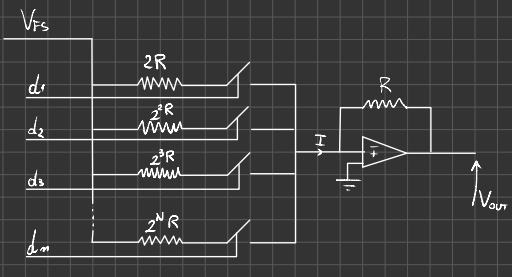
\includegraphics[width=\textwidth]{Images/figure37.png}
\end{center}
Questo convertitore presenta un \textbf{insieme di resistori di valore multiplo} (potenza di 2) di un valore \textbf{R}.
\begin{equation*}
    V_{out} = \sum \frac{V_i}{2^i} \cdot V_R
\end{equation*}
Le \textbf{resistenze} sono alimentate da una \textbf{tensione di riferimento} all'ingresso dell'\textbf{amplificatore} \textbf{operazionale}, che a sua volta in ingresso presenta una \textbf{resistenza infinita}, per cui tutta la corrente che arriva in ingresso arriva in uscita.\\ \\
In \textbf{ingresso abbiamo i bit, che pilotano gli interruttori}.\\
(1 chiuso, 0 aperto)
\section{Convertitore R-2-R}
\begin{center}
    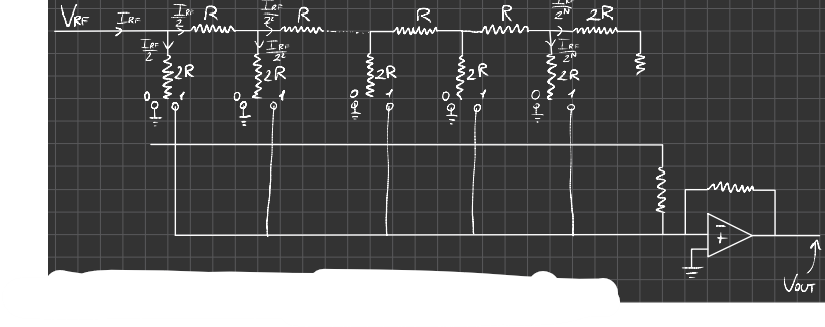
\includegraphics[width=\textwidth]{Images/figure38.png}
\end{center}
In questo convertitore, facendo una banale osservazione di \textbf{serie} e \textbf{paralleli}, possiamo dire che la \textbf{corrente} è:
\begin{equation}
    I_{in}= \frac{V_R}{2R}
\end{equation}
In particolare, la \textbf{caratteristica ingresso-uscita} di questo convertitore è la \textbf{stessa} del convertitore a \textbf{resistenze pesate}:
\begin{equation}
   V_{out} =  I_{in} R= \frac{V_R}{2}
\end{equation}
